\chapter{Application Design \& Implementation}
\label{chap:ch4}

 \par This chapter presents the design and implementation of the MSA Detector, a web application that can detect the antipatterns described in the theoretical part and represents a proof of concept to assist developers in writing code with an improved quality. The chapter begins with a high-level system overview and technology stack summary, followed by the data model design. The backend implementation is described, covering the REST API, analysis pipeline orchestration, and security layer. The frontend implementation is then presented, followed by the deployment configuration.


\section{System Overview}
\label{sec:system-overview}

\par The MSA Detector follows a client-server architecture with three main components: a Spring Boot backend that exposes a RESTful API \cite{Fielding2000}, an Angular\footnote{\url{https://angular.dev/}} single-page application (SPA) that provides the user interface, and a PostgreSQL\footnote{\url{https://www.postgresql.org/}} relational database for persistent storage. All components are containerized using Docker \cite{Merkel2014} and orchestrated via Docker Compose, as can be seen in figure~\ref{fig:architecture-overview}.

\begin{figure}
    \centering
    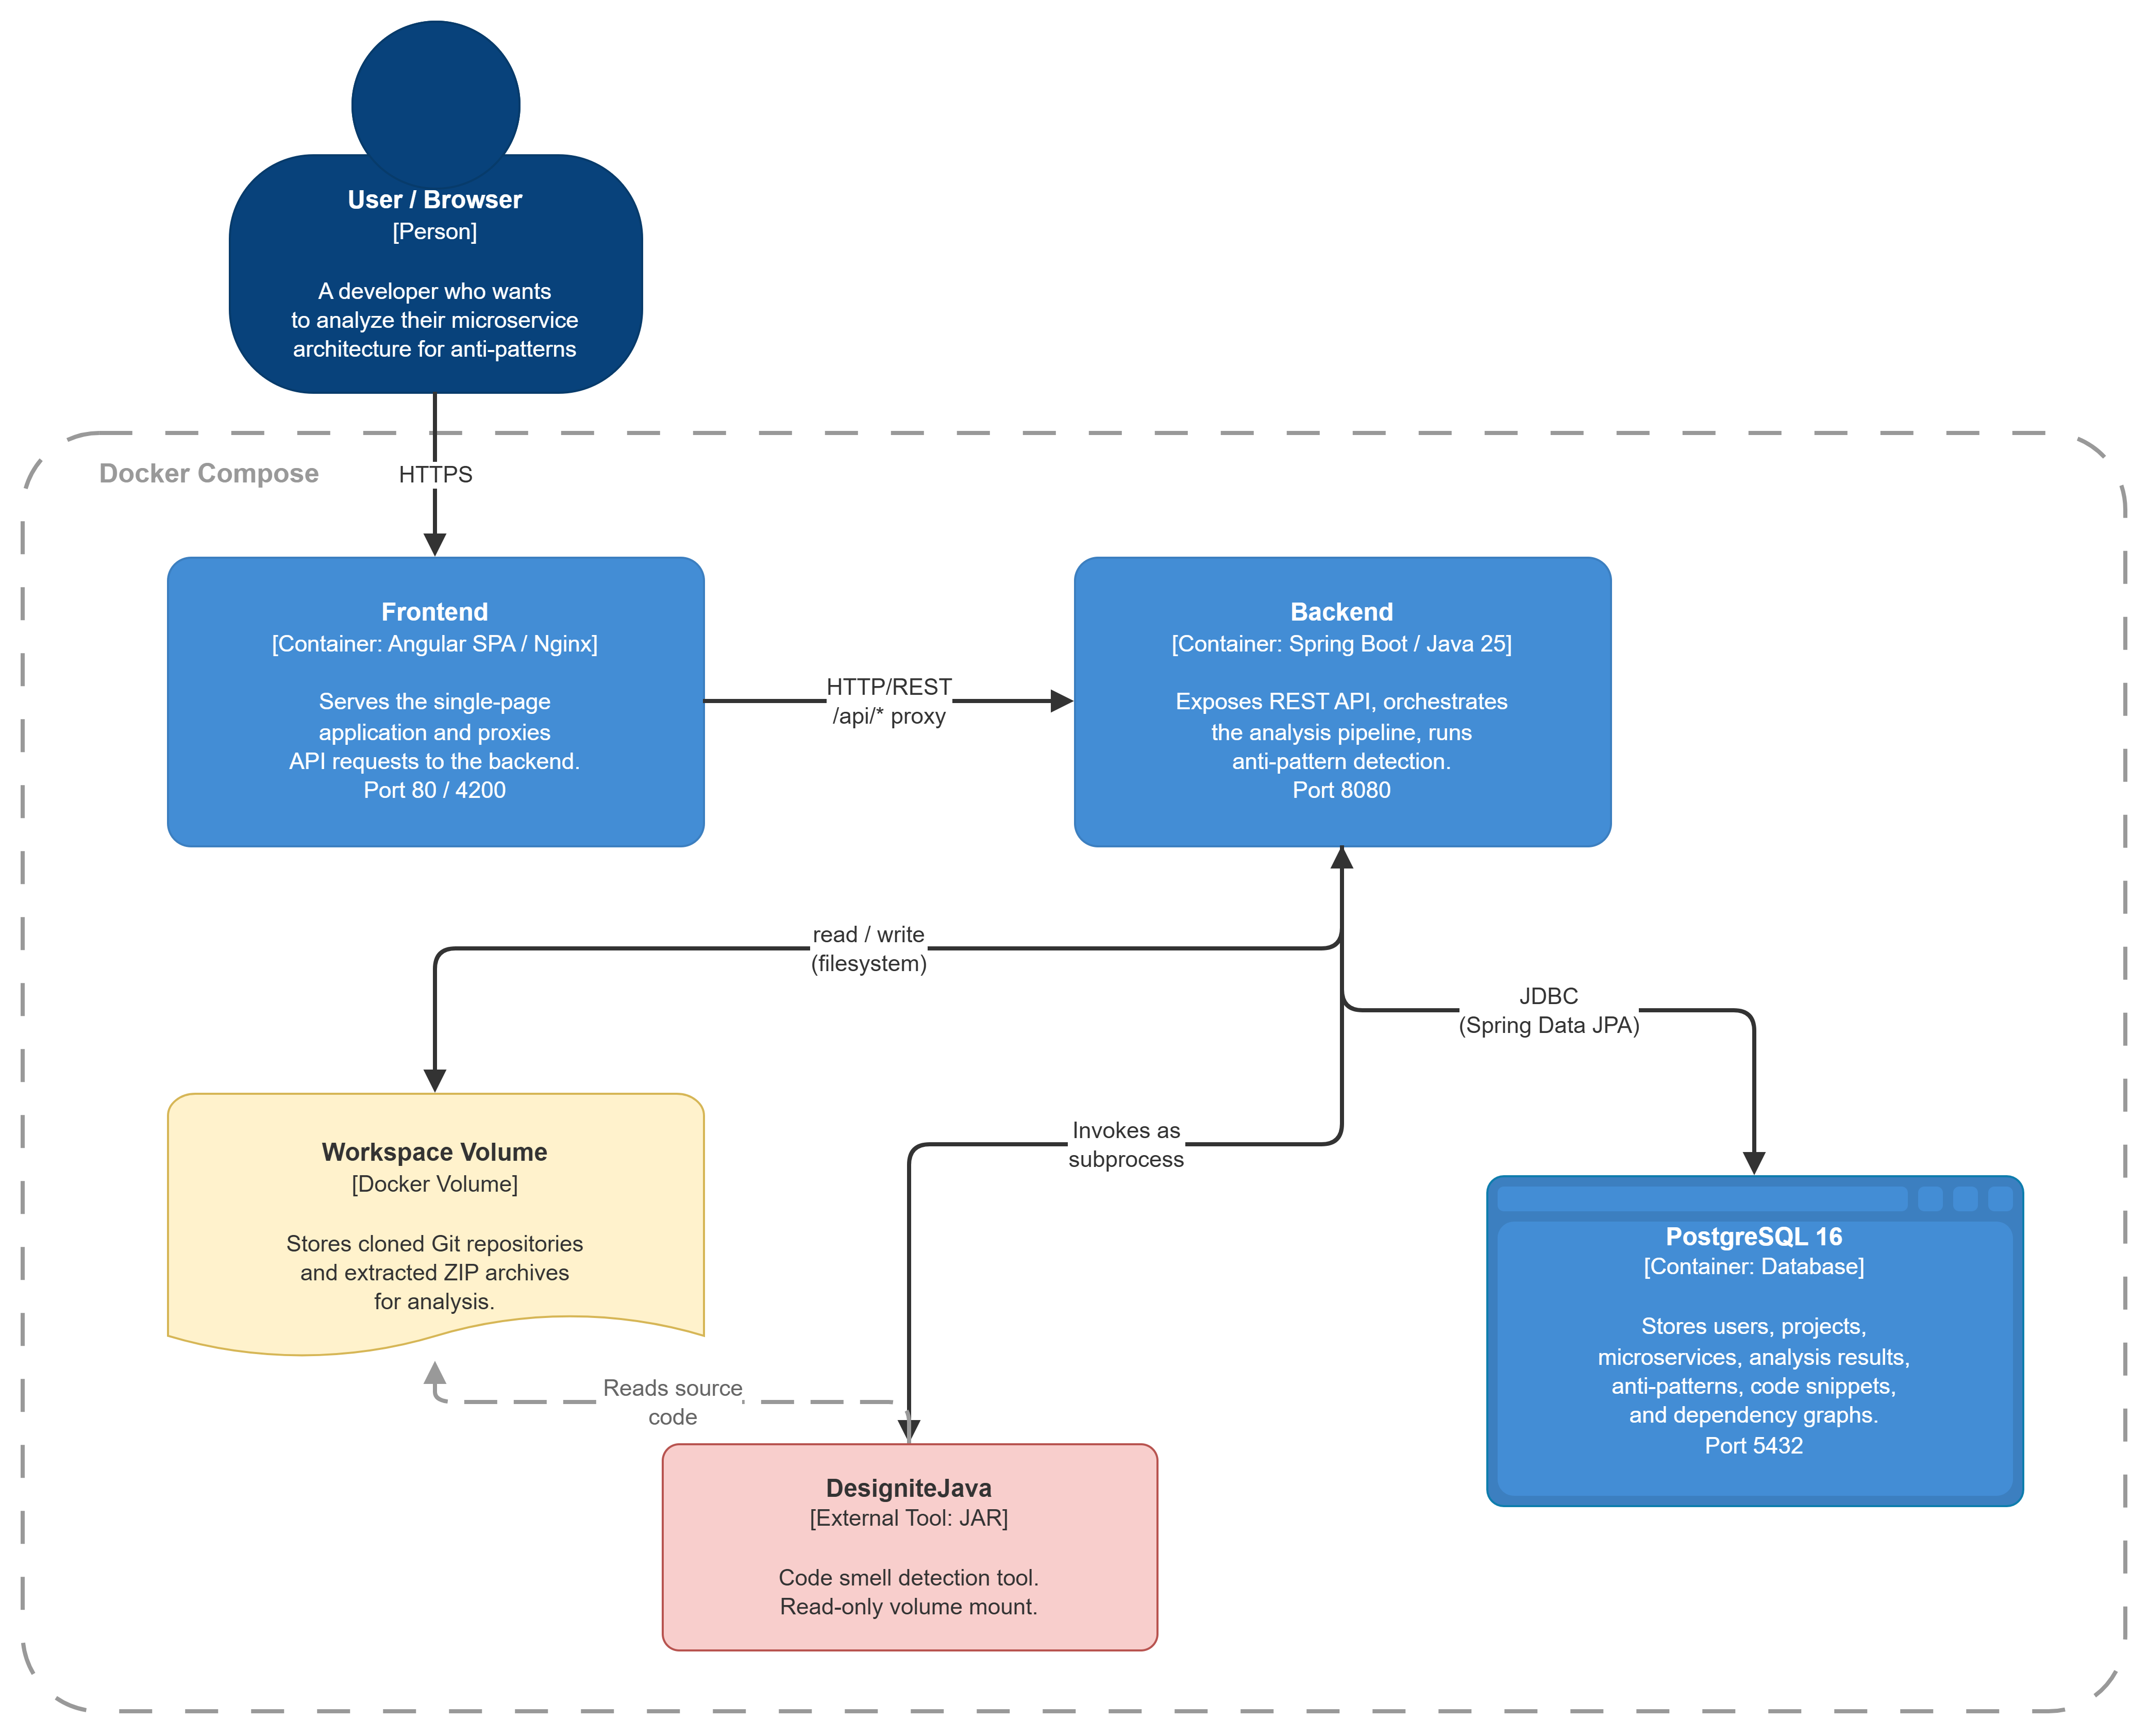
\includegraphics[scale=0.1]{figures/images/chapter4/high-level-diagram.drawio.png}
    \caption{High-level architecture of the MSA Detector system. The Angular frontend communicates with the Spring Boot backend over HTTP/REST. The backend persists data in PostgreSQL and performs analysis on cloned/uploaded source code stored on the filesystem. All components run as Docker containers orchestrated via Docker Compose.}
    \label{fig:architecture-overview}
\end{figure}

The system supports two modes of project ingestion: users can either upload a ZIP archive containing a microservices project, or provide a public GitHub/GitLab repository URL to be cloned. Once uploaded, the analysis pipeline runs asynchronously, detecting microservices boundaries, running static analysis, building the inter-service dependency graph, and detecting anti-patterns. Results are persisted and made available through the API, including a composite health score, detected anti-patterns with evidence and a dependency graph visualization.

\subsection{Technology Stack}
\label{subsec:tech-stack}

\subsubsection{DesigniteJava}
\label{subsec:designite-java}

 \par DesigniteJava is a command-line tool that performs design smell detection on Java projects \cite{Sharma2018}. It accepts a source directory as input and produces CSV files containing detected smells. In this dissertation, it is invoked as a Java subprocess with configurable timeout settings.

Table~\ref{tab:tech-stack} summarizes the technologies used in each layer of the system.

% MapStruct 1.6.3, DTO mapping
\begin{table}[htbp]
    \centering
    \footnotesize
    \begin{tabular}{|l|l|l|}
        \hline
        \textbf{Layer}                  & \textbf{Technology}                               & \textbf{Purpose}                      \\
        \hline\hline
        \multirow{8}{*}{Backend}        & Java 25, Spring Boot 4.0                          & Application framework                 \\
        \cline{2-3}
        & Spring Data JPA, Hibernate                        & ORM and data access                   \\
        \cline{2-3}
        & Spring Security, JWT (jjwt 0.12.6) \cite{RFC7519} & Authentication and authorization      \\
        \cline{2-3}
        & Spoon 11.1.0 \cite{Pawlak2016}                    & AST-based Java source code analysis   \\
        \cline{2-3}
        & DesigniteJava \cite{Sharma2018}                   & Code smell detection                  \\
        \cline{2-3}
        & JGit 7.1.0                                        & Git repository cloning                \\
        \cline{2-3}
        & Flyway                                            & Database schema migrations            \\
        \cline{2-3}
        & Lombok 1.18.38                   & Boilerplate reduction \\
        \hline
        \multirow{2}{*}{Frontend}       & Angular 19                                        & Single-page application framework     \\
        \cline{2-3}
        & TypeScript                                        & Programming language                  \\
        \hline
        Database                        & PostgreSQL 16                                     & Relational data storage               \\
        \hline
        \multirow{2}{*}{Infrastructure} & Docker, Docker Compose                            & Containerization and orchestration    \\
        \cline{2-3}
        & Eclipse Temurin 25 (Alpine)                       & JDK/JRE base images                   \\
        \hline
        API Doc               & SpringDoc OpenAPI 2.7.0                           & Swagger UI and OpenAPI spec           \\
        \hline
        Testing                         & JUnit 5, Mockito, Testcontainers 1.20.4            & Unit and integration testing          \\
        \hline
    \end{tabular}
    \caption{Technology stack summary for the MSA Detector system.}
    \label{tab:tech-stack}
\end{table}


\section{Data Model}
\label{sec:data-model}

 \par The persistent data model consists of nine entities managed via JPA and stored in PostgreSQL. All entities extend a common \texttt{BaseEntity} superclass that provides an auto-generated primary key (\texttt{id}), a creation timestamp (\texttt{created\_at}) and a last-modified timestamp (\texttt{updated\_at}) via JPA auditing. The database schema is defined and versioned using Flyway migrations.

\begin{figure}
    \centering
    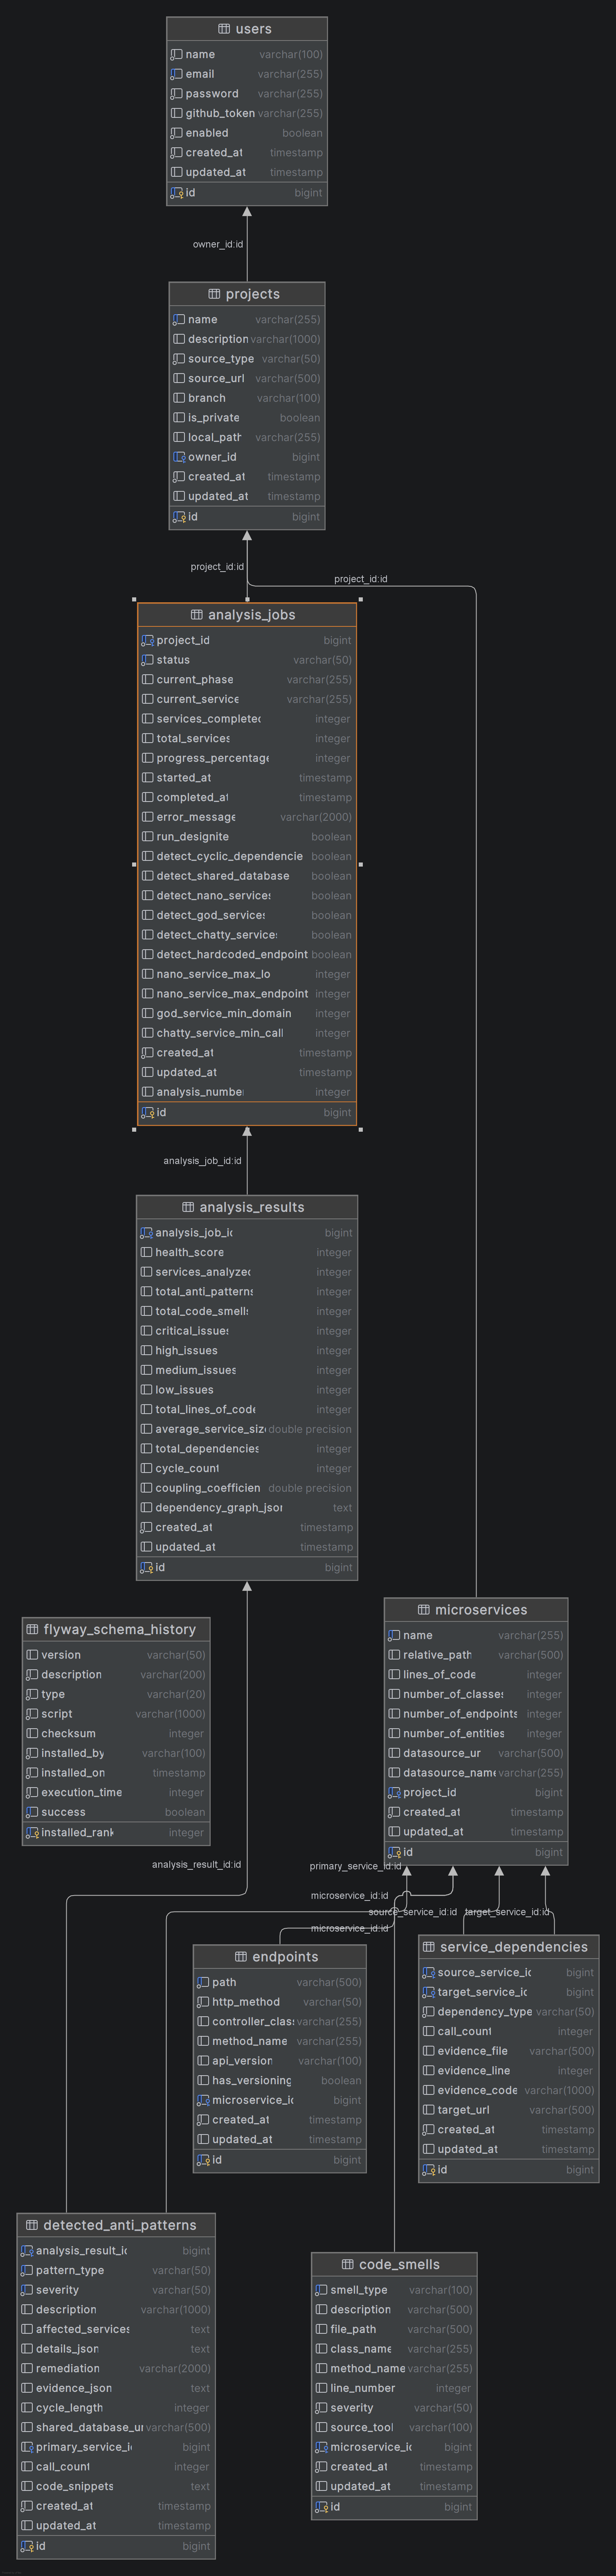
\includegraphics[scale=0.1]{figures/images/chapter4/er-diagram-modified.png}
    \caption{Entity-relationship diagram of the persistent data model, showing the nine JPA entities and their associations.}
    \label{fig:er-diagram}
\end{figure}

\subsection{Entity Descriptions}
\label{subsec:entity-descriptions}

Table~\ref{tab:entities} provides an overview of each entity and its role in the system. The relationships between entities are described below.

\begin{table}[htbp]
    \centering
    \footnotesize
    \begin{tabular}{|l|p{9cm}|}
        \hline
        \textbf{Entity}              & \textbf{Description}                                                                                                                                                                                                                                                                                                                                                                                                          \\
        \hline\hline
        \texttt{User}                & Registered user with name, email, hashed password, and optional GitHub token. Owns zero or more projects.                                                                                                                                                                                                                                                                                                                     \\
        \hline
        \texttt{Project}             & A microservice project with a name, source type (\texttt{GITHUB}, \texttt{GITLAB}, or \texttt{UPLOAD}), optional source URL and branch, and local filesystem path. Owned by a user. Contains zero or more microservices and analysis jobs.                                                                                                                                                                                    \\
 \hline
        \texttt{Microservice}        & A detected microservice within a project. Stores the service name, relative path, lines of code, number of classes, number of endpoints, datasource configuration, detection confidence level (\texttt{HIGH}, \texttt{MEDIUM}, or \texttt{LOW}), and detection signal (e.g.\ \texttt{framework-entry-point}, \texttt{dockerfile}).                                                                                                                                                                                                                                                        \\
        \hline
        \texttt{Endpoint}            & A REST endpoint detected within a microservice. Stores the URL path, HTTP method, controller class, method name, and API versioning information.                                                                                                                                                                                                                                                                              \\
        \hline
        \texttt{ServiceDependency}   & A directed dependency edge between two microservices. Stores the dependency type (e.g., \texttt{FEIGN\_CLIENT}, \texttt{REST\_TEMPLATE}, \texttt{WEB\_CLIENT}), call count, and evidence (file path, line number, code snippet, target URL).                                                                                                                                                                                  \\
        \hline
        \texttt{CodeSmell}           & A code smell detected within a microservice by DesigniteJava. Stores the smell type, severity, file path, class name, method name, and line number.                                                                                                                                                                                                                                                                           \\
        \hline
        \texttt{AnalysisJob}         & Represents a single analysis execution for a project. Tracks the job status through its lifecycle (\texttt{PENDING} $\to$ \texttt{DETECTING\_SERVICES} $\to$ \texttt{ANALYZING\_SERVICES} $\to$ \texttt{BUILDING\_GRAPH} $\to$ \texttt{DETECTING\_PATTERNS} $\to$ \texttt{COMPLETED} or \texttt{FAILED}), progress percentage, configurable detection flags and thresholds, and the analysis number for re-analysis tracking. \\
        \hline
        \texttt{AnalysisResult}      & The output of a completed analysis job. Stores aggregate metrics (health score, services analyzed, total anti-patterns, code smell count, issue counts by severity, total LOC, average service size, dependency count, cycle count, coupling coefficient) and the dependency graph as a JSON string. Has a one-to-one relationship with \texttt{AnalysisJob}.                                                                 \\
        \hline
        \texttt{DetectedAntiPattern} & An individual anti-pattern instance found during analysis. Stores the anti-pattern type, severity, human-readable description, affected services (JSON), remediation advice, evidence (JSON), and type-specific fields such as cycle length, shared database URL, call count, and code snippets (JSON).                                                                                                                       \\
        \hline
    \end{tabular}
    \caption{Overview of the data model entities.}
    \label{tab:entities}
\end{table}

\subsection{Entity Relationships}
\label{subsec:entity-relationships}

 \par The entity relationships form a hierarchical structure with the \texttt{User} entity as root. A \texttt{User} owns multiple \texttt{Project} entities (one-to-many), with cascade delete removing all projects when a user is deleted. Each \texttt{Project} contains multiple detected \texttt{Microservice} entities and multiple \texttt{AnalysisJob} entities, both with cascade delete and orphan removal. A \texttt{Microservice} entity exposes zero or more \texttt{Endpoint} entities, maintains outgoing \texttt{ServiceDependency} edges to other microservices and contains \texttt{CodeSmell} records. Each \texttt{ServiceDependency} references both a source and a target \texttt{Microservice}, representing a directed edge in the dependency graph. Every completed \texttt{AnalysisJob} produces exactly one \texttt{A\-nal\-y\-sisResults} (one-to-one), which contains zero or more \texttt{DetectedAntiPattern} instances. A \texttt{DetectedAntiPattern} optionally references a primary \texttt{Micro\-service} for service-scoped anti-patterns such as Nano Service or God Service.

All foreign key relationships use \texttt{ON DELETE CASCADE} at the database level, thus ensuring that deleting a project removes all associated microservices, endpoints, dependencies, code smells, analysis jobs, results and detected anti-patterns.


\section{Backend Implementation}
\label{sec:backend-impl}

 \par The backend is implemented as a Spring Boot application structured into the standard layers: controllers (REST API), services (business logic), repositories (data access), entities (domain model), DTOs (data transfer objects) and cross-cutting concerns (security, configuration, exception handling).

\subsection{REST API Design}
\label{subsec:rest-api}

 \par The backend exposes a RESTful API \cite{Fielding2000} under the \texttt{/api} prefix. The API is organized into three controller groups, summarized in Table~\ref{tab:api-endpoints}.

\begin{table}[htbp]
    \centering
    \footnotesize
    \begin{tabular}{|l|l|p{6cm}|}
        \hline
        \textbf{Endpoint}          & \textbf{Method} & \textbf{Description}                             \\
        \hline\hline
        \multicolumn{3}{|c|}{\textbf{Authentication} (\texttt{/api/auth})} \\
        \hline
        \texttt{/register}         & POST            & Register a new user                              \\
        \hline
        \texttt{/login}            & POST            & Authenticate and obtain JWT token                \\
        \hline
        \texttt{/me}               & GET             & Get current authenticated user info              \\
        \hline\hline
        \multicolumn{3}{|c|}{\textbf{Projects} (\texttt{/api/projects})} \\
        \hline
        \texttt{/upload}           & POST            & Upload ZIP and trigger analysis                  \\
        \hline
        \texttt{/clone}            & POST            & Clone Git repo and trigger analysis              \\
        \hline
        \texttt{/}                 & GET             & List all projects for current user               \\
        \hline
        \texttt{/\{id\}}           & GET             & Get project details                              \\
        \hline
        \texttt{/\{id\}}           & DELETE          & Delete project and all associated data           \\
        \hline
        \texttt{/\{id\}/history}   & GET             & Get full analysis history with diffs             \\
        \hline
        \texttt{/\{id\}/reanalyze} & POST            & Re-analyze project (optionally switch source)    \\
        \hline
        \texttt{/\{id\}/reupload}  & POST            & Upload new ZIP for existing project              \\
        \hline\hline
        \multicolumn{3}{|c|}{\textbf{Jobs} (\texttt{/api/jobs})} \\
        \hline
        \texttt{/\{id\}}           & GET             & Get job status and progress                      \\
        \hline
        \texttt{/\{id\}/results}   & GET             & Get analysis results with health score breakdown \\
        \hline
        \texttt{/\{id\}/diff}      & GET             & Get diff against previous analysis               \\
        \hline
        \texttt{/recent}           & GET             & Get 20 most recent jobs for current user         \\
        \hline
        \texttt{/\{id\}/cancel}    & POST            & Cancel a running job                             \\
        \hline
    \end{tabular}
    \caption{REST API endpoints exposed by the backend.}
    \label{tab:api-endpoints}
\end{table}

All endpoints except \texttt{/api/auth/**}, Swagger UI, and the actuator health endpoint require JWT authentication. Request and response payloads use Java \texttt{record} DTOs serialized to JSON via Jackson, with null fields excluded from responses.

\subsection{Authentication and Security}
\label{subsec:auth-security}

 \par The system uses stateless JWT based authentication \cite{RFC7519}. The security layer is built on Spring Security and consists of five components. The \texttt{SecurityConfig} class configures stateless session management, disables CSRF protection (the token-based API does not rely on cookies), and defines the authorization rules: public endpoints such as \texttt{/api/auth/**}, Swagger UI, and the actuator health check are exempted from authentication, while all other requests require a valid token. The \texttt{JwtTokenProvider} component generates and validates tokens using the HMAC-SHA algorithm \cite{RFC4634} - each token encodes the user ID and email as claims and carries a configurable expiration (default: 24 hours).

On every incoming request, the \texttt{JwtAuthenticationFilter}, a \texttt{Once\-Per\-Re\-questFil\-ter}, extracts the JWT from the \texttt{Authorization: Bearer} header, delegates to the provider for validation, loads the corresponding user details via the \texttt{Cus\-tomU\-serDe\-tailsSer\-vice} and populates the Spring \texttt{ SecurityContext}. If no valid token is present, the \texttt{JwtAuthenticationEntryPoint} returns a \texttt{401 Un\-au\-thor\-ized} response. Passwords are hashed using BCrypt \cite{Provos1999}, and the authenticated user's identity is injected into controller methods via the \texttt{@Au\-then\-ti\-ca\-tionPrin\-ci\-pal} annotation, which provides a \texttt{UserPrincipal} object containing the user's ID, name, and email.

\subsection{Project Ingestion}
\label{subsec:project-ingestion}

\par The web application supports two modes of project ingestion, both handled by the \texttt{ProjectService}.

\par Users may upload a ZIP archive via a multipart form data request. The file is validated (must be a ZIP, non-empty, under 500 MB), extracted to a project specific directory under the configured workspace path and normalized to handle archives that contain a single root directory. The file structure is protected against path traversal attacks (zip slip \footnote{\href{https://maven.apache.org/security-plexus-archiver.html}{Zip slip}}) by verifying that all extracted paths remain within the target directory.

\par Conversely, users can provide a public GitHub or GitLab HTTPS URL and an optional branch name. The URL is validated against a whitelist pattern. The \texttt{Git\-Clone\-Ser\-vice} uses JGit to perform a shallow clone (\texttt{depth=1}) of the repository, which downloads only the latest commit to minimize bandwidth and disk usage. A configurable timeout (default: 300 seconds) prevents indefinite blocking.

Both methods create a \texttt{Project} entity and an \texttt{AnalysisJob} entity, then trigger the asynchronous analysis. To ensure data consistency, the asynchronous worker is not started immediately, instead, it is registered through Spring's \texttt{Tran\-sac\-tionSyn\-chron\-i\-zation.afterCommit()} callback, which guarantees that the job entity is fully committed to the database before the analysis thread begins reading it. For re-analysis, the application supports re-cloning a Git repository, in order to pick up new commits, re-uploading a new ZIP file, or switching the project's source type entirely (e.g. from upload to Git repository).

\subsection{Analysis Pipeline Orchestration}
\label{subsec: analysis-pipeline}

 \par The analysis pipeline is orchestrated by the \texttt{AnalysisWorker} service, which executes asynchronously via Spring's \texttt{@Async} mechanism backed by a configurable thread pool (core size 2, maximum 5). The pipeline proceeds through five phases, each updating the job's status and progress for real-time tracking by the frontend. Listing~\ref{lst:analysis-worker} shows the top-level orchestration method.

\begin{figure}[htbp]
    \begin{minted}[
        bgcolor=darculaBg,
        style=monokai,
        fontsize=\small,
        linenos=true,
        breaklines=true,
    ]{java}
@Async
public void processJob(Long jobId) {
    AnalysisJob job = jobRepository.findByIdWithProject(jobId)
                                   .orElse(null);
    if (job == null) return;
    try {
        progressUpdater.startJob(jobId);
        Project project = job.getProject();
        Path projectPath = Path.of(project.getLocalPath());

        // Phase 1: Detect microservices
        List<Microservice> microservices =
            detectMicroservices(project, projectPath);

        // Phase 2: Analyze each service with DesigniteJava
        for (Microservice ms : microservices) {
            if (job.isRunDesignite())
                designiteService.analyzeService(ms, ...);
        }

        // Phase 3: Build inter-service dependency graph
        antiPatternDetector.buildDependencyGraph(project);

        // Phase 4: Detect anti-patterns
        AnalysisResult result =
            antiPatternDetector.detectAntiPatterns(project, job);

        // Phase 5: Persist result and mark job complete
        progressUpdater.completeJob(jobId, result);
    } catch (Exception e) {
        progressUpdater.failJob(jobId, e.getMessage());
    }
}
    \end{minted}
    \caption{Simplified \texttt{AnalysisWorker.processJob()} method showing the five-phase analysis pipeline. Each phase updates job progress for frontend polling.}
    \label{lst:analysis-worker}
\end{figure}


In the first phase, Microservice Detection (\texttt{DETECTING\_SERVICES}), the \texttt{MicroserviceDetector} identifies service boundaries using the deployability gate described in Chapter~\ref{chap:ch3}, Section~\ref{subsec:microservice-detection}. The detector first scans the project directory for build files (\texttt{pom.xml}, \texttt{build.gradle}, \texttt{build.gradle.kts}) to assemble a set of candidate modules, filtering out non-service directories (e.g.\ examples, tests, documentation, benchmarks, build support modules, and templates) using an exclusion keyword set matched against full directory names, as well as ancestor directory names. Root-level and nested aggregator modules that declare submodules are also excluded. Each surviving candidate is then evaluated against a three-signal deployability gate: framework entry point annotations such as \texttt{@SpringBootApplication} (HIGH confidence), Dockerfile presence (MEDIUM confidence), and a \texttt{public static void main()} method (LOW confidence). Only candidates that pass at least one signal are accepted as microservices; when all candidates are gated out, a fallback strategy retains the single candidate or the project root. For each detected microservice, a \texttt{Microservice} entity is created with the service name, relative path, lines of code count (computed by recursively walking all \texttt{.java} files), and the detection confidence level and signal that triggered inclusion.

The second phase, Intra-Service Analysis (\texttt{ANALYZING\_SERVICES}), invokes DesigniteJava as a subprocess for each microservice when enabled. The service passes the microservice's source directory to DesigniteJava, which produces the following CSV output files: \texttt{DesignSmells.csv}, \texttt{ImplementationSmells.csv}, and \texttt{ArchitectureSmells.csv}.
These files are parsed line by line and the detected smells are stored as \texttt{CodeSmell} entities with severity levels mapped from the smell type. The number of classes is extracted from the \texttt{TypeMetrics.csv} output. A configurable timeout (default: 1800 seconds) prevents runaway hanging subprocesses. Progress is reported per-service, allowing the frontend to display which service is currrently being analyzed and what fraction is complete.

During the third phase, Dependency Graph Construction (\texttt{BUILDING\_GRAPH}), the \texttt{DependencyGraphBuilder} scans each microservice's source code using the Spoon static analysis library \cite{Pawlak2016} to extract REST endpoints, parse datasource configuration from \texttt{application.yml} and \texttt{application.properties} and detect inter-service calls via \texttt{@FeignClient}, \texttt{RestTemplate}, and \texttt{WebClient}. The target resolution strategy, described in detail in Chapter~\ref{chap:ch3}, Section~\ref{subsec:graph-analysis}, uses the exact name matching, port-based matching and fuzzy substring matching to resolve call targets to actual microservices. The resulting \texttt{Endpoint} and \texttt{Ser\-viceDe\-pen\-den\-cy} entities are persisted to the database.

The fourth phase, Anti-Pattern Detection (\texttt{DETECTING\_PATTERNS}), delegates to the \texttt{AntiPatternDetectorService}, which orchestrates all registered detectors (see Section~\ref{subsec:detector-architecture}). Each detector is invoked in sequence, receiving the project and the list of microservices, then returning a list of \texttt{DetectedAntiPattern} instances. Failed detectors are logged and skipped, ensuring that a failure in one does not abort the entire analysis.

Finally, in the Result Assembly phase, summary statistics are computed (e.g. total lines of code, average service size, coupling coefficient (see Chapter ~\ref{chap:ch3}, Equation~\ref{eq:coupling-coefficient}), issue counts by severity) and the health score is calculated following the methodology described in Chapter~\ref{chap:ch3}, Section~\ref{subsec:health-score}. The dependency graph is serialized to a JSON structure containg nodes (services with metadata) and edges (dependencies with type and weight). The \texttt{AnalysisResult} entity is persisted, and the job status is set to \texttt{COMPLETED}.

If any phase fails, the exception is caught, the job status is set \texttt{FAILED} with the error messsage and the failure is logged. Users may also cancel a running job via the API, which sets the status to \texttt{CANCELLED}. The \texttt{JobProgressUpdater} service provides atomic progress updates by executing each update in an independent transaction (\texttt{Propagation.REQUIRES\_NEW}), thus ensuring that progress changes are immediately visible to polling clients regardless of the outer analysis transaction.

\subsection{Anti-Pattern Detector Architecture}
\label{subsec:detector-architecture}

 \par The anti-pattern detection subsystem follows the Strategy design patterns \cite{Gamma1994}. All detectors implement the \texttt{AntiPatternDetector} interface, which defines a single \texttt{detect(Project, List<Microservice>)} method returning a list of \texttt{DetectedAntiPattern} instances. Spring auto-collects all implementations via \texttt{List<AntiPatternDetector>} dependency injection.

A \texttt{BaseDetector} abstract class provides shared utility methods for JSON serialization, string truncation and source code snippet extraction. The snippet extraction method reads a configurable number of context lines above and below a target line number from the source file, producing a map with the file path, highlighted line, and surrounding code. This evidence is stored as JSON in the \texttt{De\-tec\-tedAn\-tiPa\-ttern} entity and rendered by the frontend to give developers immediate insight into the detected issue.

Table~\ref{tab:detectors} lists all ten implemented detectors. The detection algorithms for each anti-pattern were described in Chapter~\ref{chap:ch3}. New detectors can be added by implementing the interface and annotating the class with \texttt{@Component}. Spring's dependency injection automatically discovers and registers them with the orchestrator, requiring no changes to the \texttt{AntiPatternDetectorService}.

\begin{table}[htbp]
    \centering
    \footnotesize
    \begin{tabular}{|l|l|l|}
        \hline
        \textbf{Detector Class}              & \textbf{Anti-Pattern}  & \textbf{Severity} \\
        \hline\hline
        \texttt{SharedDatabaseDetector}      & Shared Database        & HIGH              \\
        \hline
        \texttt{CyclicDependencyDetector}    & Cyclic Dependency      & CRITICAL          \\
        \hline
        \texttt{NanoServiceDetector}         & Nano Service           & MEDIUM            \\
        \hline
        \texttt{GodServiceDetector}          & God Service            & HIGH              \\
        \hline
        \texttt{ChattyServiceDetector}       & Chatty Service         & HIGH              \\
        \hline
        \texttt{HardcodedEndpointDetector}   & Hardcoded Endpoints    & MEDIUM            \\
        \hline
        \texttt{DistributedMonolithDetector} & Distributed Monolith   & CRITICAL          \\
        \hline
        \texttt{ApiVersioningDetector}       & API Versioning Absence & MEDIUM            \\
        \hline
        \texttt{WrongCutsDetector}           & Wrong Cuts             & HIGH               \\
        \hline
        \texttt{EsbMisuseDetector}           & ESB Misuse             & HIGH                \\
        \hline
    \end{tabular}
    \caption{Implemented anti-pattern detectors with their target patterns and default severity levels. The detection algorithms for each anti-pattern were described in Chapter~\ref{chap:ch3}.}
    \label{tab:detectors}
\end{table}

\subsection{Analysis Diff (Re-Analysis Comparison)}
\label{subsec:analysis-diff}

 \par When a project is re-analyzed, the backend computes a diff between the current and previous analysis results, inspired by SonarQube's "Clean as You Code" concept \cite{SonQ}. The \texttt{AnalysisDiffService} compares two \texttt{AnalysisResult} instances and produces an \texttt{AnalysisDiffResponse} DTO.

The diff includes the health score delta, previous versus current score and letter grade, as well as per-metric deltas for all aggregate metrics: total anti-patterns, code smells, issues by severity, total lines of code, services analyzed, cycle count, dependency count and coupling coefficient. Anti-pattern changes are categorized in three groups: \textit{resolved} anti-patterns that were present in the previous analysis but absent in the current one, \textit{new} anti-patterns detected for the first time, and \textit{unchanged} anti-patterns that were still found in the later runs. The diff also computes per-category score deltas for each of the four health score categories (Anti-Patterns, Code Quality, Architecture, Service Sizing). Finally, a human-readable summary string is generated (e.g., ''Health improved from 52~(D)~$\to$~78~(C). 2~anti-patterns resolved, 1~new.''), providing a short assessment of the changes.

The diff is automatically embedded in the analysis results response and is also available through a dedicated \texttt{GET /api/jobs/\{id\}/diff} endpoint. The project history endpoint returns all completed analyses ordered from the newest first, each paired with its diff against the predecessor, thus providing a full timeline view of architectural evolution.

\subsection{Exception Handling}
\label{subsec:exception-handling}

 \par A global exception handler (\texttt{GlobalExceptionHandler}) annotated with Spring's \texttt{@RestControllerAdvice} provides a centralized error handling across all controllers. The handler translated domain exceptions into structured JSON error responses with a consistent format containing an error code, a human-readable message, and a timestamp. \texttt{ResourceNotFoundException} maps to \texttt{404 Not Found}; \texttt{InvalidFileException} and \texttt{IllegalArgumentException} map to \texttt{400 Bad Request}; \texttt{IllegalStateException} maps to \texttt{409 Conflict} for operations on resources in an invalid state (e.g., cancelling an already-completed job); \texttt{Bad\-Cre\-den\-tialsEx\-cep\-tion} maps to \texttt{401 Unauthorized}; and \texttt{Me\-thodAr\-gu\-mentNotVa\-lidEx\-ception} maps to \texttt{400 Bad Request} with per-field validation messages. A catch-all handler logs unexpected exceptions at error level and returns a generic \texttt{500 Internal Server Error} to avoid leaking stack traces.

\subsection{Testing}
\label{subsec:testing}

\par The backend is accompanied by a suite of unit and integration tests built with JUnit~5 and Mockito. Each of the ten anti-pattern detectors has a dedicated test class that verifies detection logic in isolation: repository dependencies are mocked, and temporary directories (\texttt{@TempDir}) provide realistic file-system fixtures where needed. The tests cover positive detection, negative (no-detection) scenarios, boundary conditions on configurable thresholds, and correct propagation of metadata such as severity, affected services and code snippets. Shared utility methods in \texttt{BaseDetector} (JSON serialization, snippet extraction, string truncation) are tested through a concrete subclass that exposes the protected API. Controller-level integration tests use Spring's \texttt{@WebMvcTest} slice to verify HTTP status codes, request validation, JSON response structure and security constraints via \texttt{MockMvc}, with service-layer beans replaced by Mockito mocks. A separate test-profile \texttt{application.yml} configures an in-memory context with Hibernate's \texttt{create-drop} schema strategy, shorter timeouts and reduced logging, allowing the full test suite to run without an external database.


\section{Frontend Implementation}
\label{sec:frontend-impl}

 \par The frontend is implemented as an Angular single-page application (SPA) written in TypeScript. It communicates with the backend exclusively through the REST API described in Section~\ref{subsec:rest-api}. This section describes the application structure, key pages, reusable components and the authentication integration.

\subsection{Application Structure and Routing}
\label{subsec:frontend-structure}

 \par The frontend is built with Angular 19 and uses the framework's standalone component architecture - the application contains no \texttt{NgModule} declarations. Every component, page, interceptor and guard is defined as a standalone unit that declares its own imports, simplifying the dependency graph and enabling fine-grained tree-shaking at build time. The application is bootstrapped in \texttt{main.ts} via Angular's \texttt{bootstrapApplication} function, which registers the router and the HTTP client together with the authentication and error interceptors.

The source tree is organized into five directories under \texttt{src/app/}: \texttt{pages/} contains five page-level components, each corresponding to a route; \texttt{components/} contains seven reusable presentational components; \texttt{services/} contains two singleton services (\texttt{ApiService}, which encapsulates all HTTP calls to the backend, and \texttt{AuthService}, which manages JWT-based authentication state); \texttt{interceptors/} contains two functional HTTP interceptors; \texttt{guards/} contains a single route guard; and \texttt{models/} provides a barrel file exporting all TypeScript interfaces. The root \texttt{AppComponent} renders a context-sensitive navigation header and a \texttt{<router-outlet>} for the active page.

Table~\ref{tab:frontend-routes} lists the route configuration. The empty path redirects to \texttt{/upload}, so authenticated users land on the upload page by default. Three of the five routes are protected by the \texttt{authGuard}, which redirects unauthenticated users to the login page.

\begin{table}[htbp]
    \centering
    \footnotesize
    \begin{tabular}{|l|l|c|}
        \hline
        \textbf{Path}            & \textbf{Component}             & \textbf{Auth Required} \\
        \hline\hline
        \texttt{/login}          & \texttt{LoginPageComponent}    & No                     \\
        \hline
        \texttt{/register}       & \texttt{RegisterPageComponent} & No                     \\
        \hline
        \texttt{/upload}         & \texttt{UploadPageComponent}   & Yes                    \\
        \hline
        \texttt{/results/:jobId} & \texttt{ResultsPageComponent}  & Yes                    \\
        \hline
        \texttt{/history}        & \texttt{HistoryPageComponent}  & Yes                    \\
        \hline
    \end{tabular}
    \caption{Frontend routing configuration. Routes marked ''Auth Required'' are protected by the \texttt{authGuard}.}
    \label{tab:frontend-routes}
\end{table}

\subsection{Authentication Integration}
\label{subsec:frontend-auth}

 \par The frontend authentication layer consists of four cooperating pieces: the \texttt{AuthService} singleton, two HTTP interceptors and a route guard. \texttt{AuthService} stores the JWT token and the serialized user object in the browser's \texttt{localStorage} and exposes the current user as a \texttt{currentUser\$} observable that the navigation bar subscribes to; it provides \texttt{login()}, \texttt{register()} and \texttt{logout()} methods that persist or clear this state, the first two posting credentials to the backend's \texttt{/api/auth} endpoints. The \texttt{authInterceptor} attaches an \texttt{Authorization: Bearer <token>} header to every outgoing request except the public \texttt{/auth/login} and \texttt{/auth/register} calls, while the \texttt{errorInterceptor} intercepts \texttt{401} responses, clears the stale session and redirects the user to the login page. Finally, the \texttt{authGuard} (a functional \texttt{CanActivateFn}) protects the \texttt{/upload}, \texttt{/results/:jobId} and \texttt{/history} routes, redirecting unauthenticated users to \texttt{/login}.

\subsection{Pages}
\label{subsec:frontend-pages}

 \par The application contains five page components, each responsible for a distinct user workflow.

\begin{figure}[htbp]
    \centering
    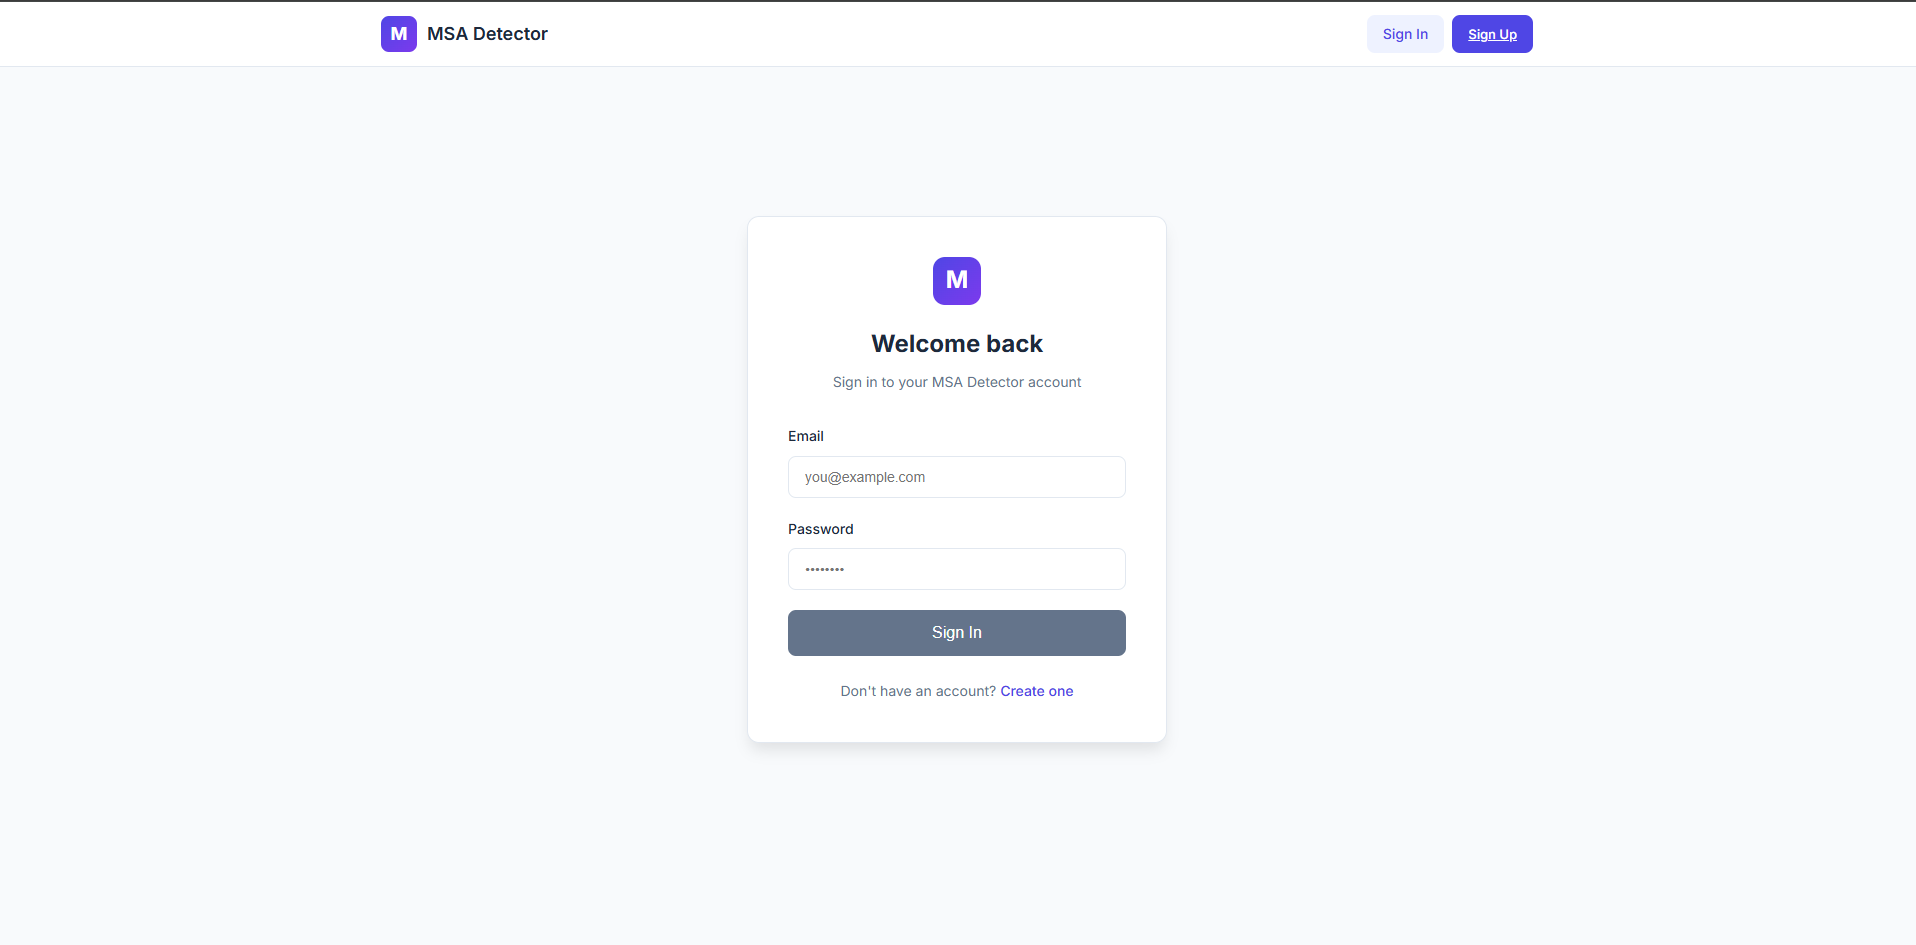
\includegraphics[scale=0.25]{figures/images/chapter4/login_page.png}
    \caption{Login page of the MSA Detector frontend.}
    \label{fig:login-page}
\end{figure}

The \texttt{LoginPageComponent} and \texttt{RegisterPageComponent} present forms bound via Angular's \texttt{FormsModule} two-way binding (\texttt{ngModel}), with a computed \texttt{canSubmit} getter that disables the submit button until the fields are populated and no request is in flight. On submission they call \texttt{AuthService.login()} or \texttt{register()}, navigate to \texttt{/upload} on success, and display the backend error message inline on failure; registration additionally enforces a minimum password length.

\begin{figure}[htbp]
    \centering
    \subfloat[\centering ZIP upload 1]{{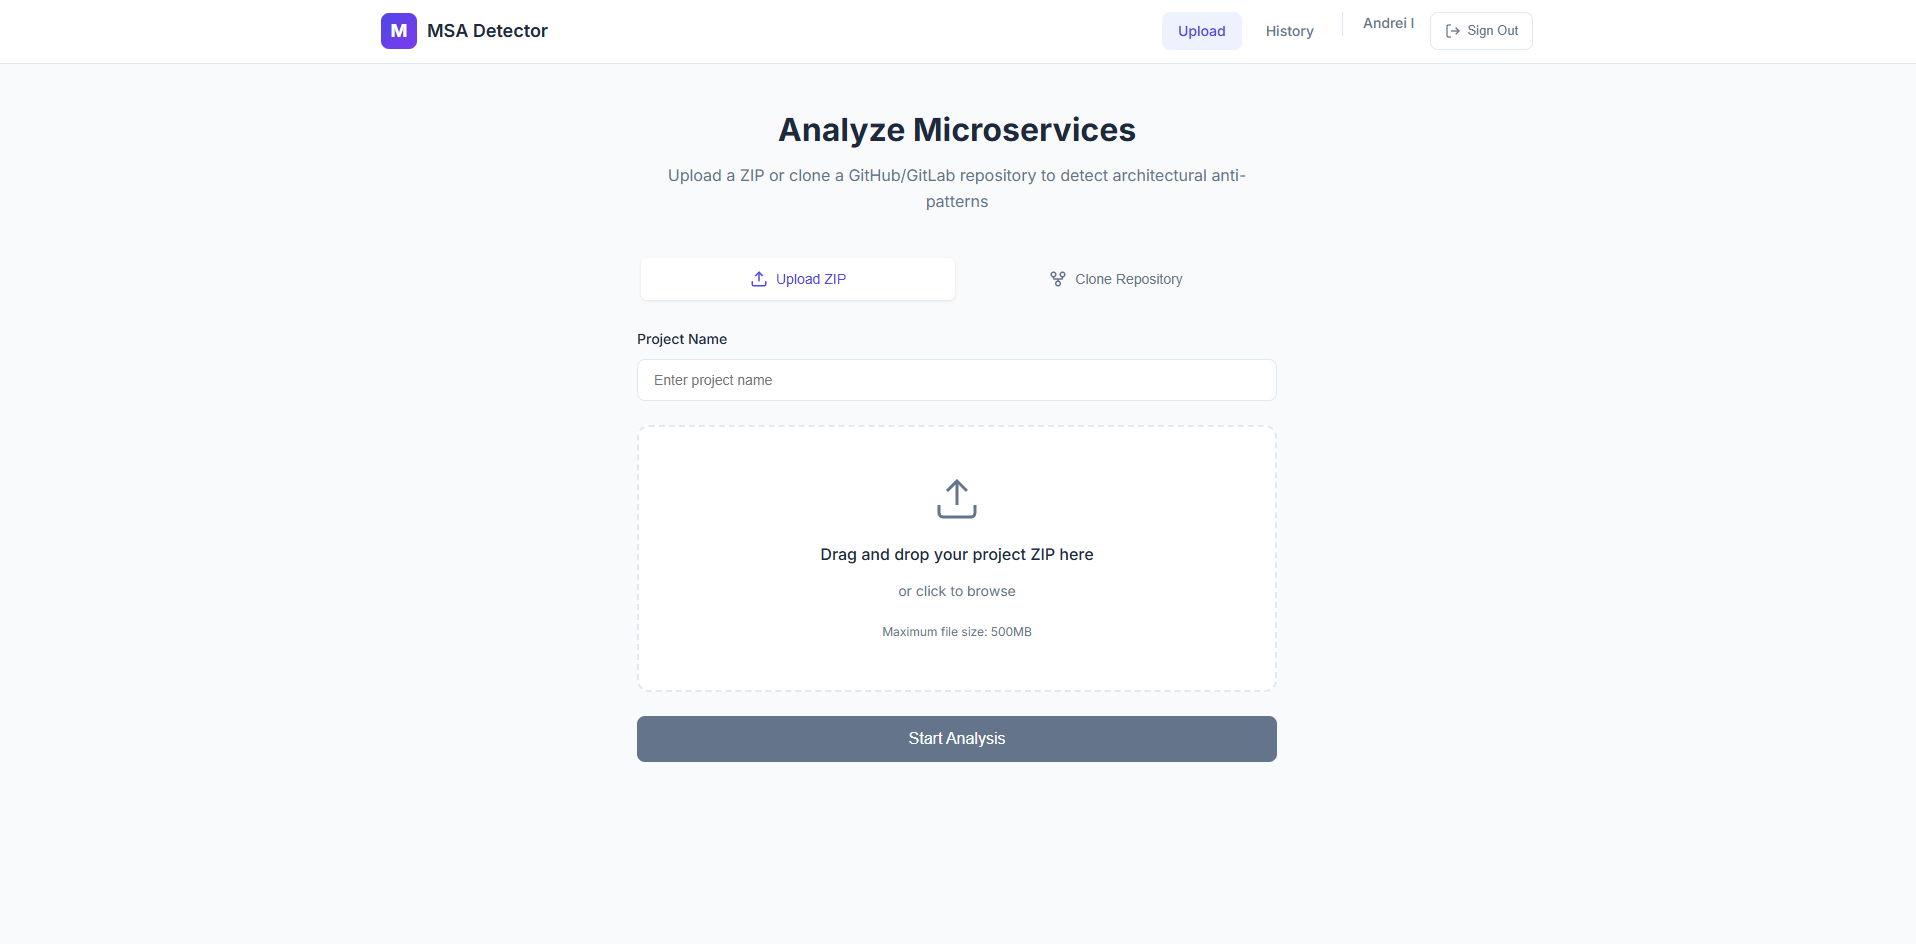
\includegraphics[width=15cm]{figures/images/chapter4/zip_page.png} }}%
    \qquad
    \subfloat[\centering Git clone 2]{{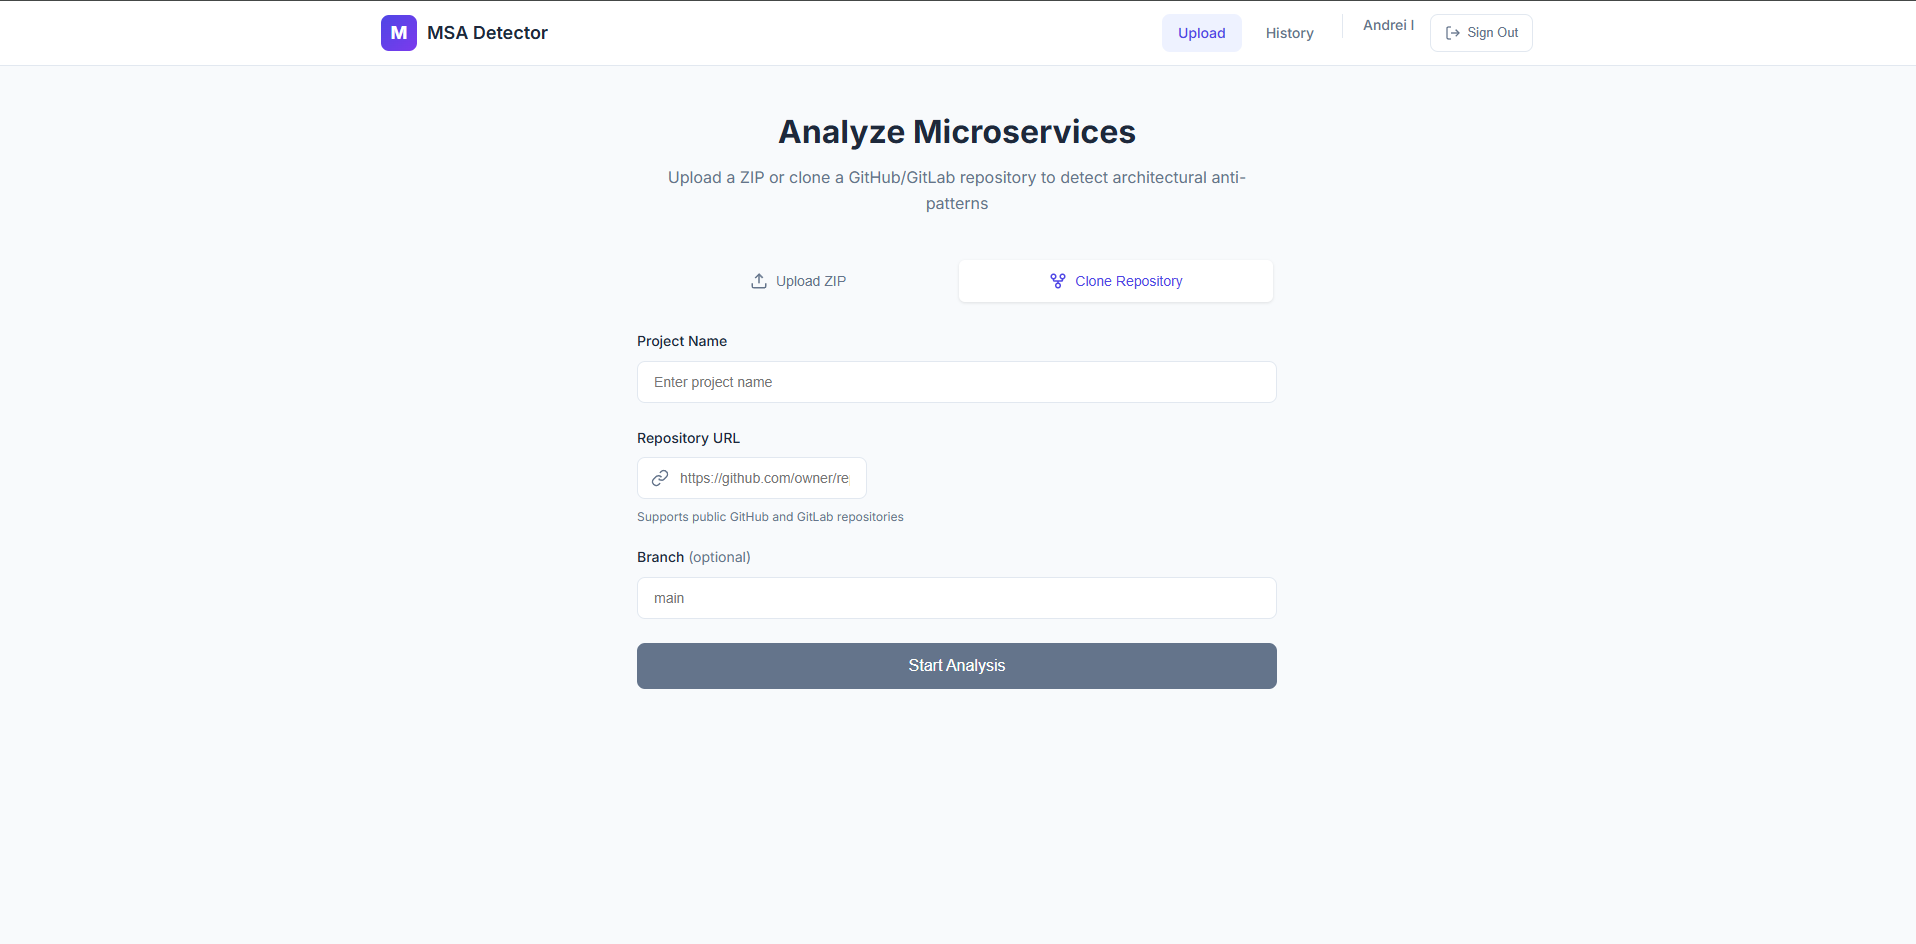
\includegraphics[width=15cm]{figures/images/chapter4/clone_page.png} }}%
    \caption{Upload page with ZIP upload (left tab) and Git clone (right tab) modes.}
    \label{fig:upload-page}
\end{figure}

The \texttt{UploadPageComponent} supports two project ingestion modes, selectable via a tab interface. In ZIP upload mode it embeds the reusable \texttt{FileUploadComponent} for drag-and-drop file selection and tracks upload progress in real time via Angular's \texttt{HttpClient} progress events; in Git clone mode it presents a client-side-validated repository URL and an optional branch field. Once the backend responds with a job ID, the page transitions to an analysis-in-progress state, embeds the \texttt{ProgressTrackerComponent} and polls \texttt{ApiService.getJobStatus()} every two seconds, navigating to the results page on completion (or showing an error on failure). The polling interval is cleared in \texttt{ngOnDestroy} to prevent memory leaks.

 \begin{figure}[htbp]
     \centering
     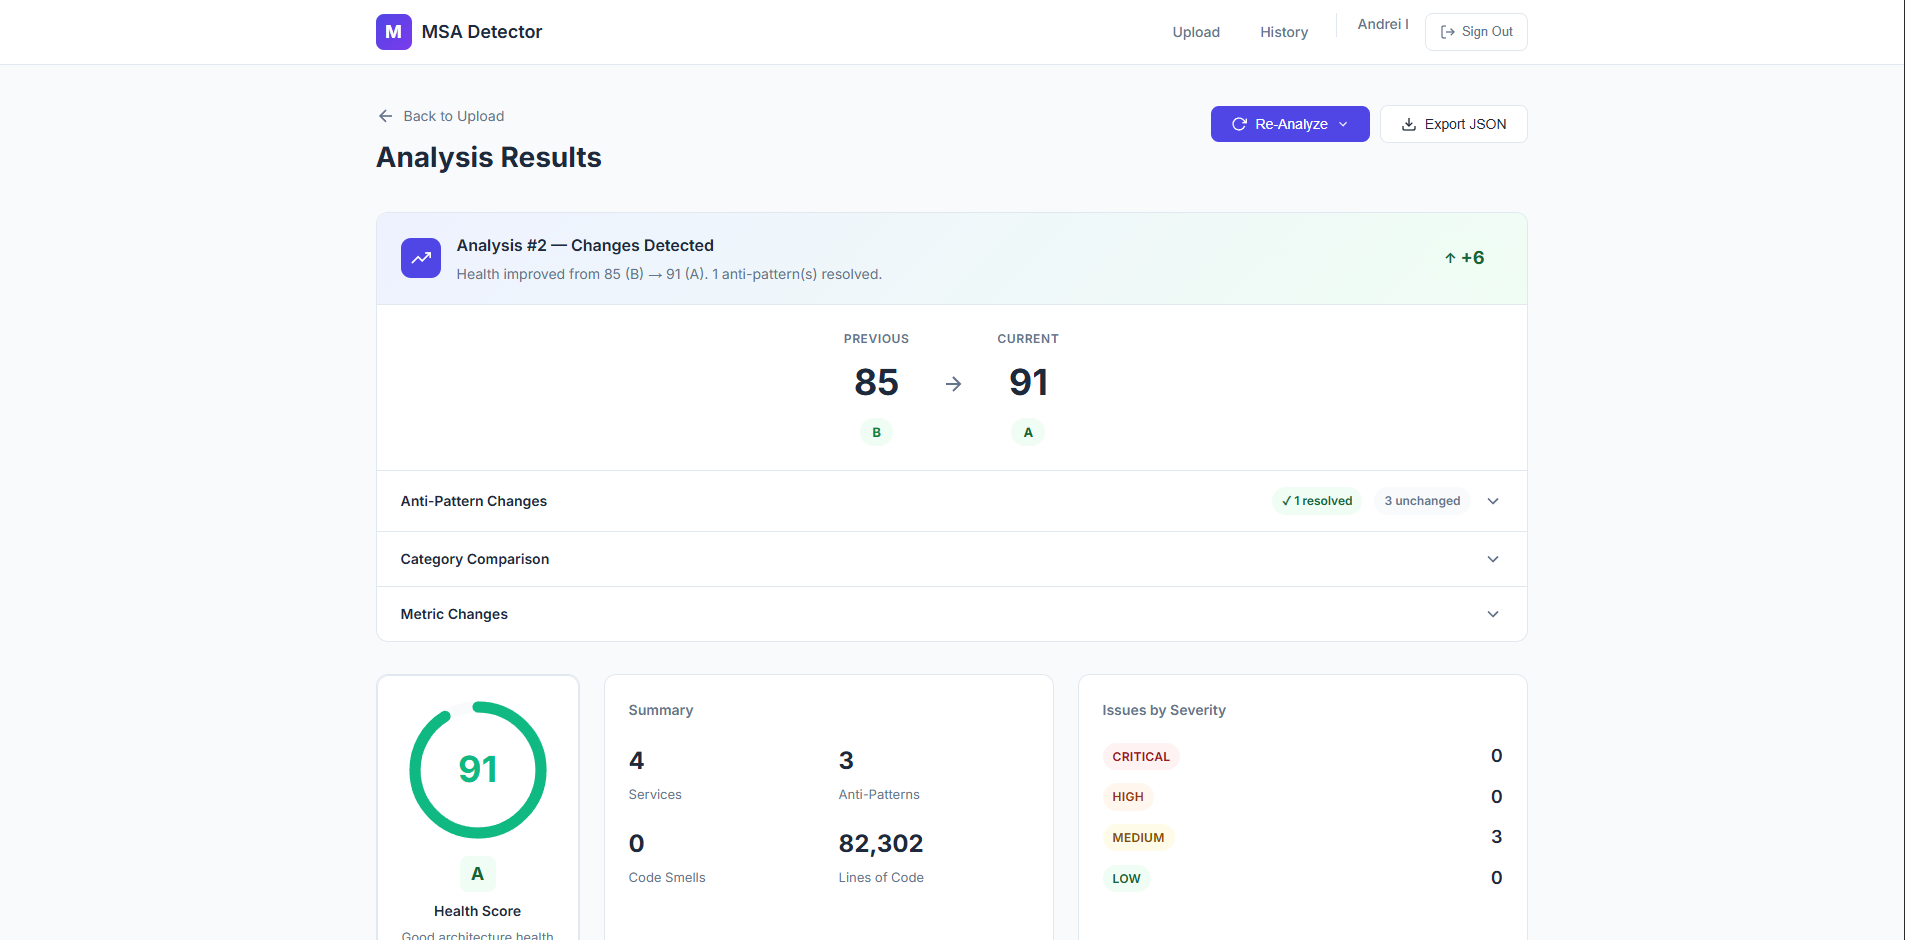
\includegraphics[scale=0.3]{figures/images/chapter4/analysis_page.png}
     \caption{Results page displaying the health score gauge, summary metrics, issues by severity, health score breakdown, detected anti-patterns, and dependency graph.}
     \label{fig:results-page}
 \end{figure}

The \texttt{ResultsPageComponent} is the primary output of the application. It loads the \texttt{AnalysisResult} for the route's \texttt{jobId} together with the job metadata and parent project. A header offers a \texttt{Re-Analyze} dropdown (new ZIP upload or clone from a different URL, each opening a modal and beginning polling of the new job) and an \texttt{Export JSON} button that downloads the serialized result. When the result contains a diff, the \texttt{DiffBannerComponent} is shown at the top; otherwise an informational note is rendered. Below this, a grid of summary cards displays the \texttt{HealthScoreComponent} gauge, key metrics (services, anti-patterns, code smells, LOC) and issue counts by severity, followed by the \texttt{HealthScoreBreakdownComponent} and a two-column grid pairing the \texttt{AntiPatternListComponent} with the interactive \texttt{DependencyGraphComponent}.

 \begin{figure}[htbp]
     \centering
     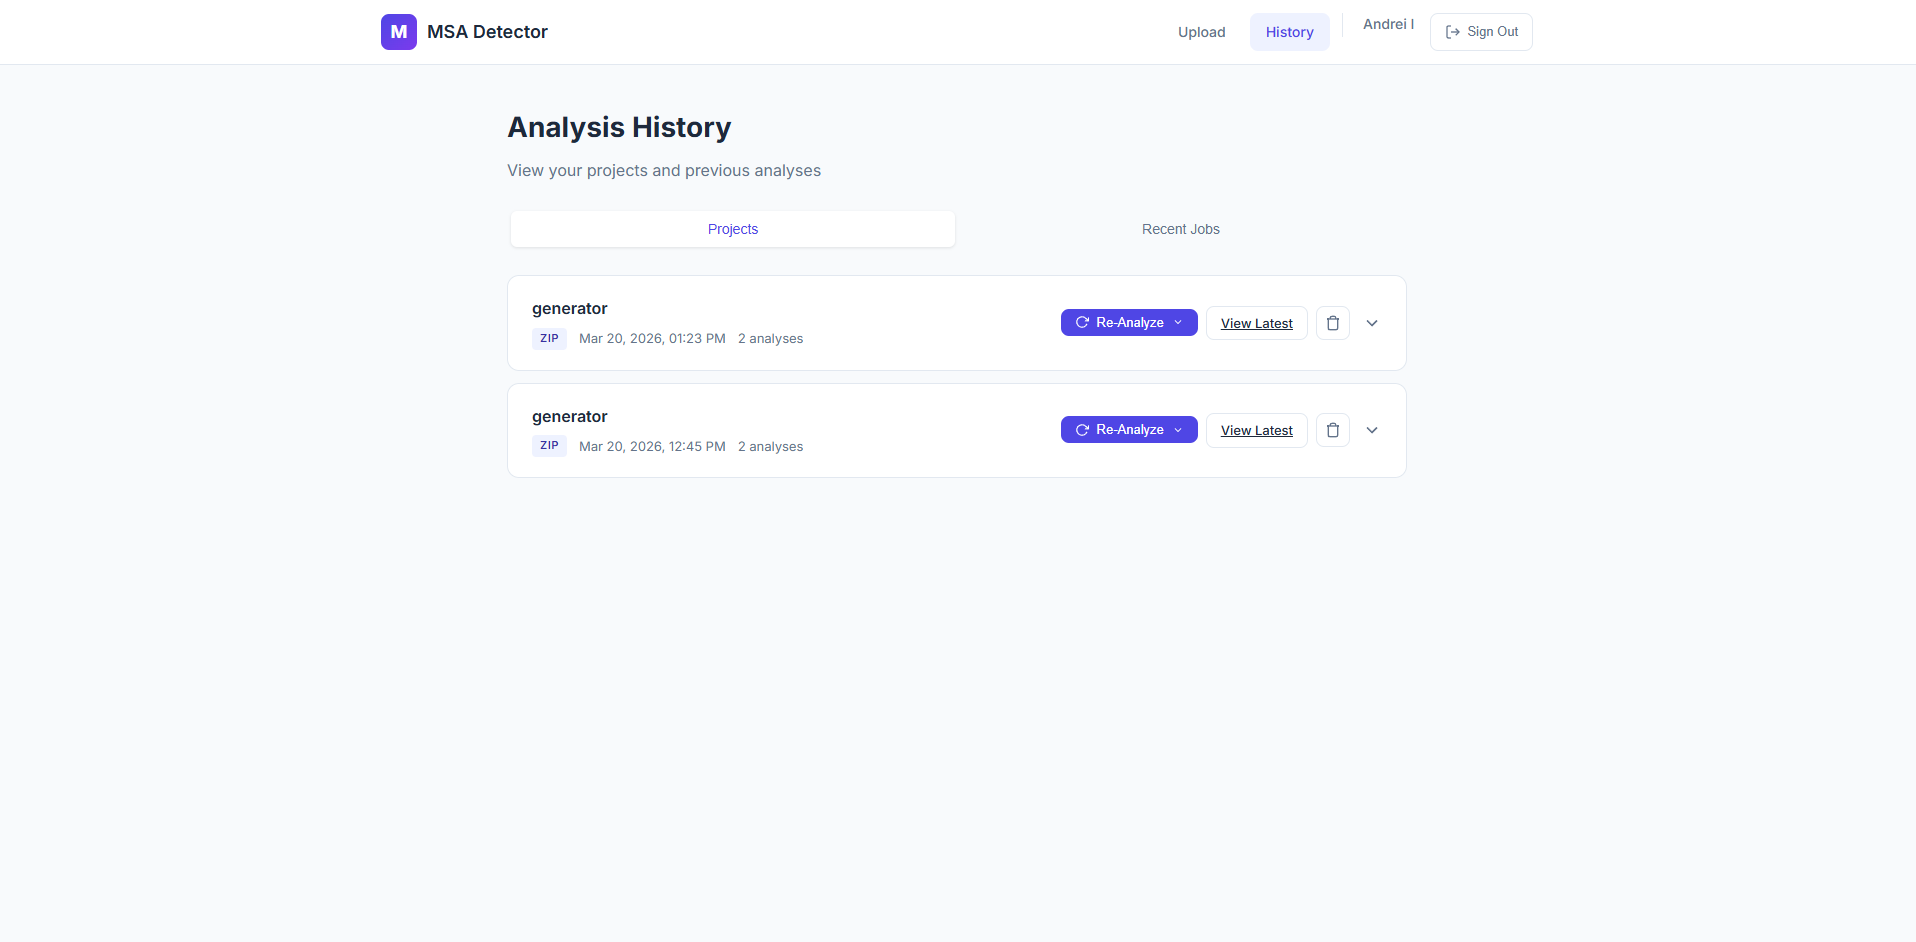
\includegraphics[scale=0.3]{figures/images/chapter4/history_page.png}
     \caption{History page showing the projects list with an expanded project's analysis timeline and diff information.}
     \label{fig:history-page}
 \end{figure}

The \texttt{HistoryPageComponent} provides an overview of all the user's projects and recent analysis jobs, organized into two tabs. The Projects tab lists each project with its source type, creation date and number of analyses; expanding a project reveals its full analysis history, each entry showing the health score, anti-pattern count and (when available) the colour-coded diff against the previous analysis, with click-through to the corresponding results page and the same re-analysis and delete options as the results page. The Jobs tab displays the 20 most recent analysis jobs with their status, analysis number and timestamps.

\subsection{Reusable Components}
\label{subsec:frontend-components}

 \par The application defines seven standalone reusable components composed into pages via Angular's input and output bindings. The \texttt{HealthScoreComponent} renders the composite score as an SVG circular gauge with a colour-coded letter-grade badge. The \texttt{HealthScoreBreakdownComponent} displays the four score categories as collapsible cards with progress bars and itemized deductions. The \texttt{DiffBannerComponent} visualizes per-metric deltas between successive analyses, supporting an \texttt{inverse} mode for metrics where a decrease is an improvement. The \texttt{DependencyGraphComponent} renders the inter-service dependency graph as an interactive, force-directed visualization using Cytoscape.js \footnote{\href{https://cytoscape.org/index.html}{Cytoscape.js}}, with node size scaled by lines of code and pan/zoom support. The \texttt{FileUploadComponent} provides a drag-and-drop ZIP selection zone, the \texttt{CodeSnippetViewerComponent} renders source-code evidence with numbered, highlighted lines, and the \texttt{ProgressTrackerComponent} shows a multi-step progress indicator reflecting the analysis pipeline's current phase. Each component is purely presentational; the polling and data-loading logic lives in the parent page components.

\section{Deployment}
\label{sec:deployment}

 \par The application is containerized using Docker and orchestrated with Docker Compose. Two configurations are provided: a development configuration for local development and a production configuration for deployment on a productive environment.

\subsection{Docker Configuration}
\label{subsec:docker-config}

 \par The backend is packaged using a multi-stage Dockerfile. The build stage uses an Eclipse Temurin JDK 25 Alpine image to compile the application with Maven; Docker's layer caching ensures dependency resolution is only re-executed when \texttt{pom.xml} changes by copying and resolving dependencies (\texttt{mvn dependency:go-offline}) before copying the source code. The runtime stage uses a minimal JRE 25 Alpine image, installs Git (required for repository cloning at runtime), creates a non-root user (\texttt{appuser}) for security and runs the application with container-aware JVM settings (\texttt{-XX:+UseContainerSupport}, \texttt{-XX:MaxRAMPercentage=75.0}) that allow the JVM to respect container memory limits. A health check endpoint (\texttt{/actuator/health}) is configured for container orchestration.

\subsection{Docker Compose (Development)}
\label{subsec:docker-dev}

 \par The development Docker Compose configuration defines four services on a shared bridge network. The PostgreSQL~16 (Alpine) container serves as the database, initialized via Flyway migration scripts \footnote{\href{https://github.com/flyway/flyway}{Flyway}} and exposed on port 5432 with a periodic health check (\texttt{pg\_isready}). The backend container is built from the Dockerfile described above, connected to the database via environment variables, and mounts the DesigniteJava JAR as a read-only volume. It is exposed on port 8080 and depends on the database being healthy before starting. The frontend container is built from the sibling \texttt{dissertation\_frontend} repository and served via Nginx on port 4200, with a startup dependency on the backend's health check. An optional pgAdmin container, enabled via the \texttt{tools} Docker Compose profile, provides a web-based database administration interface on port 5050 for development convenience. Named volumes (\texttt{postgres\_data}, \texttt{workspace\_data}) persist the database and analysis workspace across container restarts, so that uploaded projects and analysis results are not lost during container restarts.

\subsection{Docker Compose (Production)}
\label{subsec:docker-prod}

 \par The production configuration introduces several differences for security and resource management. Sensitive configuration, i.e. the database password and JWT signing secret, is injected via required environment variables (using Docker Compose's \texttt{\$\{VAR:?error\}} syntax) rather than hardcoded defaults, which prevents accidental deployment with insecure credentials. The database port is not exposed to the host, instead, only the frontend container exposes port~80 (configurable via \texttt{FRONTEND\_PORT}), acting as the single entry point to the system. The frontend's Nginx configuration reverse-proxies API requests at the \texttt{/api} path to the backend container, which eliminates the need for CORS headers and ensures that all traffic enters through a single port. Resource limits are enforced via Docker's \texttt{deploy\-.resources\-.limits}: 1\,GB for PostgreSQL, 2\,GB for the backend, and 256\,MB for the frontend. The backend's health check start period is increased to 60 seconds to accommodate longer JVM startup times in memory-constrained environments.

\subsection{Configuration Management}
\label{subsec:config-management}

 \par The application configuration is externalized via environment variables with sensible defaults for local development, following established practices for cloud-native applications \cite{Newman2015}. Spring Boot's property placeholder mechanism (\texttt{\$\{VAR:default\}}) in \texttt{application.yml} resolves environment variables at startup, with fallback values ensuring that the application runs out-of-the-box in a development environment without additional configuration. Table~\ref{tab:config-params} lists the key configurable parameters.

\begin{table}[htbp]
    \centering
    \footnotesize
    \begin{tabular}{|l|l|p{4.5cm}|}
        \hline
        \textbf{Parameter} & \textbf{Default} & \textbf{Description} \\
        \hline\hline
        \texttt{DB\_HOST} & localhost & Database hostname \\
        \hline
        \texttt{DB\_PORT} & 5432 & Database port \\
        \hline
        \texttt{DB\_NAME} & msadetector & Database name \\
        \hline
        \texttt{JWT\_SECRET} & (dev key) & JWT signing secret \\
        \hline
        \texttt{JWT\_EXPIRATION} & 86400000 (24h) & JWT token lifetime in ms \\
        \hline
        \texttt{WORKSPACE\_DIR} & /tmp/\ldots/workspace & Analysis workspace path \\
        \hline
        \texttt{DESIGNITE\_JAR\_PATH} & /opt/\ldots/DesigniteJava.jar & Path to DesigniteJava \\
        \hline
        \texttt{CLONE\_TIMEOUT} & 300 & Git clone timeout (seconds) \\
        \hline
        \texttt{ANALYSIS\_TIMEOUT} & 1800 & DesigniteJava timeout (seconds) \\
        \hline
        \texttt{NANO\_MAX\_LOC} & 500 & Nano service LOC threshold \\
        \hline
        \texttt{NANO\_MAX\_ENDPOINTS} & 2 & Nano service endpoint threshold \\
        \hline
        \texttt{GOD\_MIN\_GOD\_CLASSES} & 1 & God service minimum God Class count \\
        \hline
        \texttt{CHATTY\_MIN\_CALLS} & 10 & Chatty service call count threshold \\
        \hline
    \end{tabular}
    \caption{Key configurable parameters and their default values.}
    \label{tab:config-params}
\end{table}

\subsection{Production Deployment Considerations}
\label{subsec:prod-deployment}

 \par While the Docker Compose configurations described above are sufficient for single-server deployments, deploying the system to a publicly accessible production environment introduces additional concerns around hosting, data persistence, network security and operational maintenance. The containerized architecture is portable across any Docker-capable host: a single virtual private server (VPS) with modest resources (around 4\,GB of RAM and 2 vCPUs) can run all three containers, while higher-availability setups could use a managed container orchestration platform (e.g.\ AWS ECS, Google Cloud Run, Kubernetes) and a managed PostgreSQL service to offload backups and failover. Horizontal scaling of the backend is not required, as analysis jobs are inherently sequential per project.

 \par A key design decision simplifies operations: all analysis evidence, including the source code snippets shown to users and the dependency graph, is extracted \textit{during the analysis phase} and persisted as JSON directly in PostgreSQL (in the \texttt{code\_snippets} and \texttt{dependency\_graph\_json} columns), rather than read from the filesystem at request time. Consequently, results remain fully available even after the workspace volume is cleaned to reclaim disk space, and the database is the only stateful component that requires backup. For a public deployment, HTTPS should be enabled to protect JWT tokens in transit, either by placing a reverse proxy that handles TLS termination (e.g.\ Caddy or Traefik with Let's Encrypt certificates) in front of the stack, which otherwise exposes only port~80, or by terminating TLS at a cloud load balancer. Operationally, the PostgreSQL volume should be backed up off-host (e.g.\ scheduled \texttt{pg\_dump} to object storage such as AWS S3), and the backend's 2\,GB memory limit and five-worker analysis thread pool should be tuned to the host's resources, since heap usage is dominated by Spoon's AST analysis of large projects.

\section{Summary}
\label{sec:ch4-summary}

 \par This chapter presented the design and implementation of the MSA Detector application. The high-level architecture consists of an Angular frontend, a Spring Boot backend, and a PostgreSQL database, all containerized with Docker. The data model comprises nine entities capturing users, projects, microservices, endpoints, dependencies, code smells, analysis jobs, results, and detected anti-patterns. The backend implements a RESTful API \cite{Fielding2000} with JWT authentication \cite{RFC7519}, asynchronous analysis pipeline orchestration, a pluggable anti-pattern detector architecture based on the Strategy design pattern \cite{Gamma1994}, and a re-analysis diff feature inspired by SonarQube's \texttt{Clean As You Code} concept. A suite of unit and integration tests verifies detector logic, controller behaviour and service interactions. Deployment is managed through Docker Compose with separate development and production configurations. The chapter concluded with a discussion of production deployment considerations, noting that all analysis evidence is persisted in the database during analysis, making PostgreSQL the sole stateful component required for serving results. The next chapter evaluates the system's detection accuracy and performance on real-world open-source microservice projects.
